 \chapter{Introduction}
\label{cp.intro}

From ancient times to the modern day, astronomy has played an essential role in all cultures and eras.
Questions about the infinite cosmos and our place in it have intrigued great minds for millennia.
To answer these questions, astronomers construct instruments to tap into the cosmos' ocean of data and devise statistical methods to make inferences.
Each drop of cosmic data improves inference and takes us to the answers we seek.
However, until quite recently, astronomy has existed in a relatively data-poor environment. 
This situation has been flipped thanks to the advent of modern instruments and computers, leaving astronomers with rich datasets not easily described by traditional methods.
Some astronomers are turning to data-driven approaches to make inferences with the vast quantities of data now available.
This section takes a look back at areas of astronomy that have recently seen significant data improvements and have provided new insights into the nature of stars, planets, and even black holes.
These conversations will spark ideas and provide impetus for the rest of the thesis.



\section{Observational HR-Diagrams through the ages}

In 1872, astronomers began recording spectroscopic data for thousands of stars in the Henry Draper Catalogue~\citeme.
Antonia Maury, a female astronomer, working in the Harvard observatory, noticed that some stars in the catalog were much brighter than other stars of the same color and sorted those brighter stars into a different category from their less-luminous brethren. 
Several years later, Einjar Hertzpsrung, working on his star classification project in 1905, noticed the same thing as Maury: some stars had very similar colors but very different brightness~\citeme.
With more data available in 1913, Henry Norris Russell demonstrated the effect far more strikingly. 
Russel plotted the absolute magnitude against spectral type for Maury's stars, nearby stars with parallaxes measured at the time, stars from the open cluster Hyades, and several moving groups ($\sim200$ stars in total). 
This plot, an observational Hertzpsrung-Russel (HR) diagram, has been recreated with modern stellar data in Figure~\ref{fig:HR-diagrams}a.

\begin{figure}
\begin{center}
  \centerline{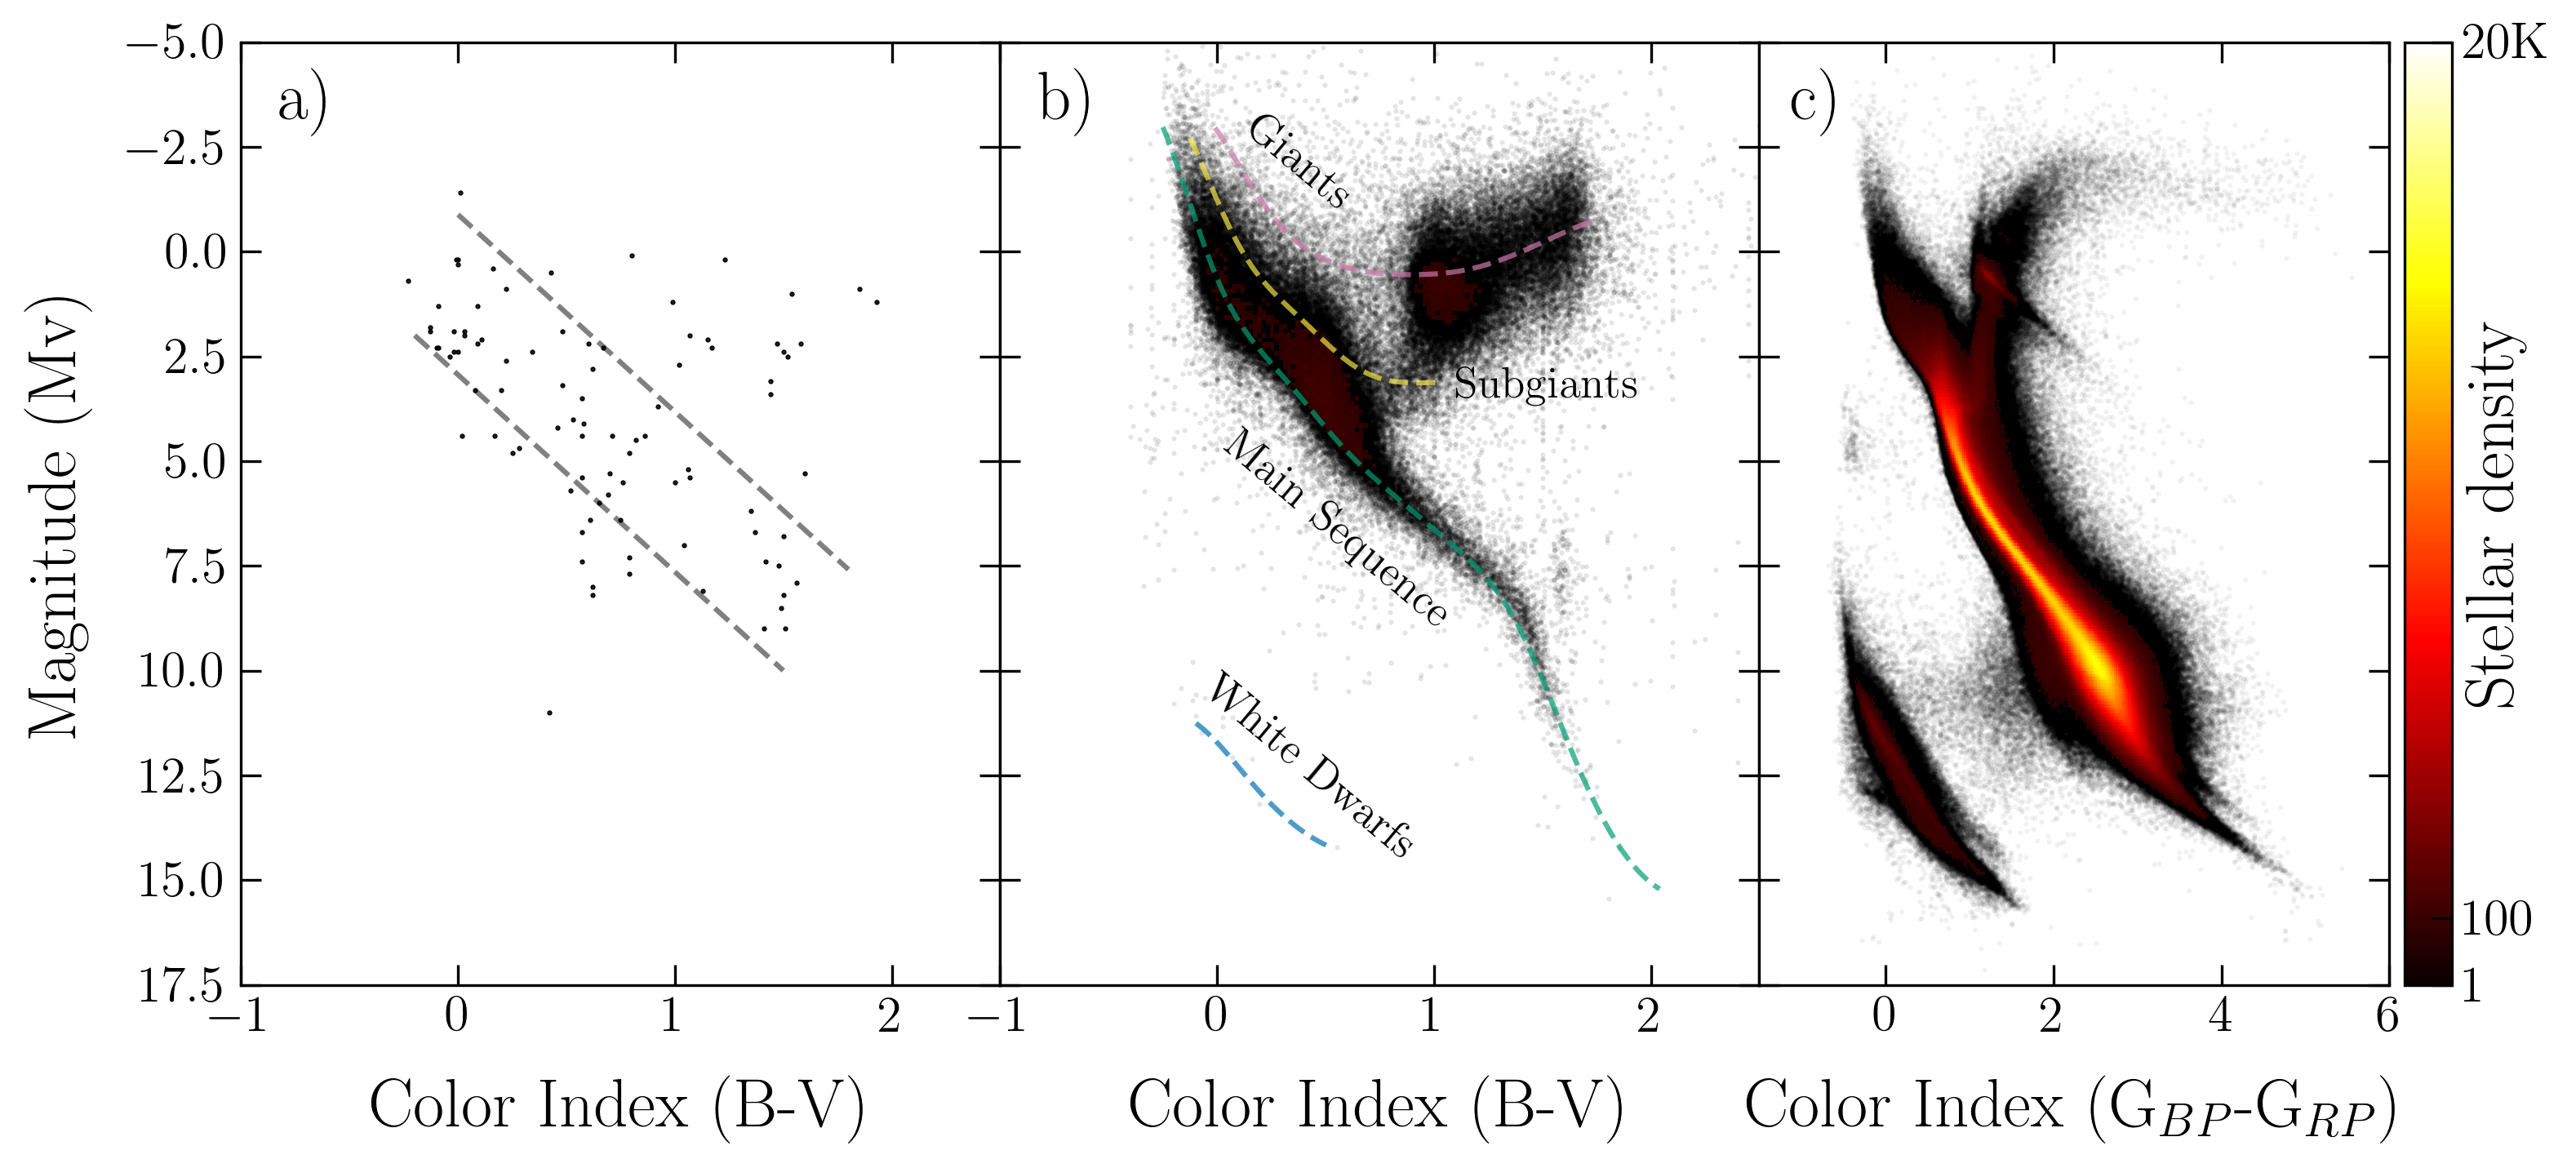
\includegraphics[width=1.2\linewidth]{figures/hr_diagram.png}}
  \caption{\textbf{Observational HR-Diagrams through the ages: Catalog stars' color index plotted on the horizontal axis and absolute magnitude on the vertical axis. Different regions of the diagram depend on the stars' masses, chemical composition, ages, and stages in the stellar life cycle. The color scale represents the number of stars in each portion of the diagram (black represents lower numbers of stars, and brighter colors correspond to increasingly higher numbers of stars). Panel (a) uses stars cataloged in 1914, panel (b) uses 1993 Hipparcos stars, and panel (c) uses 2022 Gaia stars. 
}  \github{https://github.com/avivajpeyi/hr_diagram_past_to_present}}
  \label{fig:HR-diagrams}
\end{center}
\end{figure}

The plot's data points helped Russell demonstrate that the temperature and luminosity of stars are related.
Brighter stars are displayed in the top part of the diagram, while dimmer stars are in the bottom. 
Bluer (hotter-surface) stars are on the left, and redder (cooler-surface) stars are on the right. 
Russell noted that most of the plotted stars fell in a band from the upper left to the lower right.
He indicated this region with lines (the gray dashed lines reconstructed Figure~\ref{fig:HR-diagrams}a).
Russell and Hertzsprung also noticed a separate category of bright but cool red stars in the upper right corner. 
They realized that these bright-cool red stars have a large surface area to produce high luminosity at low temperatures. 
Hertzsprung hence dubbed these as the ``giant" stars.  
Consequently, he named the less-luminous low-temperature red stars "dwarf" stars. 
Russell recognized that the red dwarfs were just the bottom end of the band of stars within the gray lines in Figure~\ref{fig:HR-diagrams}a. 
Hence, Russell extended the grouping of ``dwarf" stars to the entire sequence, the sequence now known as the ``main sequence."
Even though the plot only contained a few stars, it provided Russell with a convenient way to illustrate his ideas about stellar evolution:
\myblockquote{The giant stars then represent successive stages in the heating up of a body and must be
more primitive the redder they are; the dwarf stars represent consecutive stages in later
cooling, and the reddest of these are the farthest advanced.}{Henry Russell, 1914}

  % https://arxiv.org/pdf/1302.0862.pdf
Other astronomers like Eddington also used similar data and the HR diagram to drive some of their theories. 
For example, a decade later, Eddington's mass-luminosity relation would add evidence for stellar evolution down the main sequence.
Soon, the HR diagram became a cornerstone diagram for modern astrophysics, and the concepts of stellar categories led to various advancements in our understanding of stellar physics~\citeme. 
Fortunately, since 1914, technological advances have created much larger samples of stars with well-measured properties, further improving our understanding of stellar physics.


The European Space Agency launched Hipparcos Satellite in 1989\footnote{Hipparcos, an acronym for HIgh Precision PARallax COllecting Satellite, is also reference to Hipparchus, the ancient Greek astronomer who drew up the first accurate star map.}. 
One of the Hipparcos mission's primary goals was to provide a higher resolution observational HR diagram to obtain a detailed structure of stars with $M_v>0$ magnitude. 
In its four years of operation, this satellite cataloged nearly 120,000 stars. 
The Hipparcos catalog stars with low parallax errors, plotted in Figure~\ref{fig:HR-diagrams}b,  show many more details than those in the 1914 HR diagram. 
Firstly, the vertical arm leading off the main sequence and turning to the right is much better defined -- this is the red giant branch indicating that as massive stars get older, they swell and become brighter and redder.
Similarly, the lower left of the diagram shows the white dwarf branch. 
The white dwarf region displays where the less massive stars (like our sun) that cannot undergo a supernova as they get older end up. 
Additionally, if we plotted stars with higher parallax errors, various other categories, such as the bright and super giants, are also visible.

A few years later, Hipparcos's successor Gaia made a considerable leap by cataloging 1.8 billion stars at an accuracy 200 times better than that of Hipparcos. 
Figure~\ref{fig:HR-diagrams}c displays the Gaia stars with low parallax errors obtained in Gaia's third data release. 
This new HR diagram contains over 100 times more stars than Hippacros and allows astronomers to identify more refined details. 
For example, compare the hand full of white dwarfs in the Hipparcos diagram versus the thousands in the Gaia HR diagram.
This increase in white dwarf data has allowed astronomers to study the differences between white dwarfs made with helium cores and hydrogen cores ~\citeme. 
Another exciting detail displayed in the Gaia HR diagram is the imprint of stellar binaries.
These binaries are present both in the main sequence and the white dwarf regions of the diagram (see the second tails at slightly higher magnitudes in both the main sequence and white dwarf regions of the plot).
The Gaia HR diagram appears to have a smaller red giant branch compared to Hipparcos's HR diagram. However, the Gaia HR diagram has many more resolved features, such as the primary and secondary red clumps and the asymptotic giant branch bump. 
The sheer volume of the data made such discoveries possible! 

In addition to data on stellar temperatures and brightness, our catalogs now also contain stellar spectra and time-series data on stellar positions and proper motions.
This data has enabled astronomers to drive theoretical work and make inferences about the nature of stars.
In the following two sections of this chapter, we discuss two more fields where astronomical data has unveiled profound discoveries. 



\section{The era of Gravitational wave astronomy}

%% What is a GW 
When some stars reach the end of their lives, they can turn into compact objects such as neutron stars and black holes. 
Some compact objects give away their positions via electromagnetic (EM) radiation due to accretion. 
Others reveal themselves via gravitational wave (GW) radiation emitted due to an oscillating mass quadrupole moment.
Any system with a gravitational quadrupole changing with time produces changes in its gravitational field, resulting in the emission of energy as gravitational waves.
Gravitational-wave astronomy gives us a new tool to examine the cosmos that complements classic electromagnetic astronomy.
Using gravitational waves, we may investigate systems such as binary black holes, which are undetectable to the naked eye, and potentially get fresh understanding into objects such as neutron stars that would otherwise be inaccessible.


\subsection{A brief history of GW detection}
%% History of GW
In 1974, Russell Hulse and Joseph Taylor discovered a pulsar signal using the Arecibo radio telescope.
Measurements revealed that the pulsars' orbital period fluctuates repeatedly every few hours, indicating it is in orbit with a hidden companion.
Hulse and Taylor noted that the orbital period was decaying -- the pulsar and its companion were inspiralling.
After observing the system for another 30 years, they determined that the decrease of the orbital period was the result of the binary releasing gravitational waves, the first observation of gravitational waves.

This indirect detection of gravitational waves paved the groundwork for the Laser Interferometer Gravitational-Wave Observatory, LIGO. 
LIGO was constructed in 1999, but it was not until 2014 that the first gravitational wave from the merging of a binary black hole system was identified.
Since then, the LIGO-VIRGO-KAGRA (LVK) collaboration has recorded several petabytes of data and astronomers have discovered more than ninety gravitational wave (GW) signals from compact binary mergers.
Individually, these events have provided astronomers with interesting information about various astrophysical objects. 
Taken together, the events form a population that can be studied as a whole. 
The remainder of this section introduces the LVK collaborations efforts to 
\begin{enumerate}[i]
\item search for GW signals from compact binary mergers,
\item decode the GW signals to decipher the properties of the system that generated the signal, and 
\item study ``demographics'' of the merging black hole populations.
\end{enumerate}
This thesis touches on these broad categories, illustrated in Figure~\ref{fig:gw_pipeline}. 
This section provides some more background for each of the main topics covered. 

\begin{figure}
\begin{center}
  \centerline{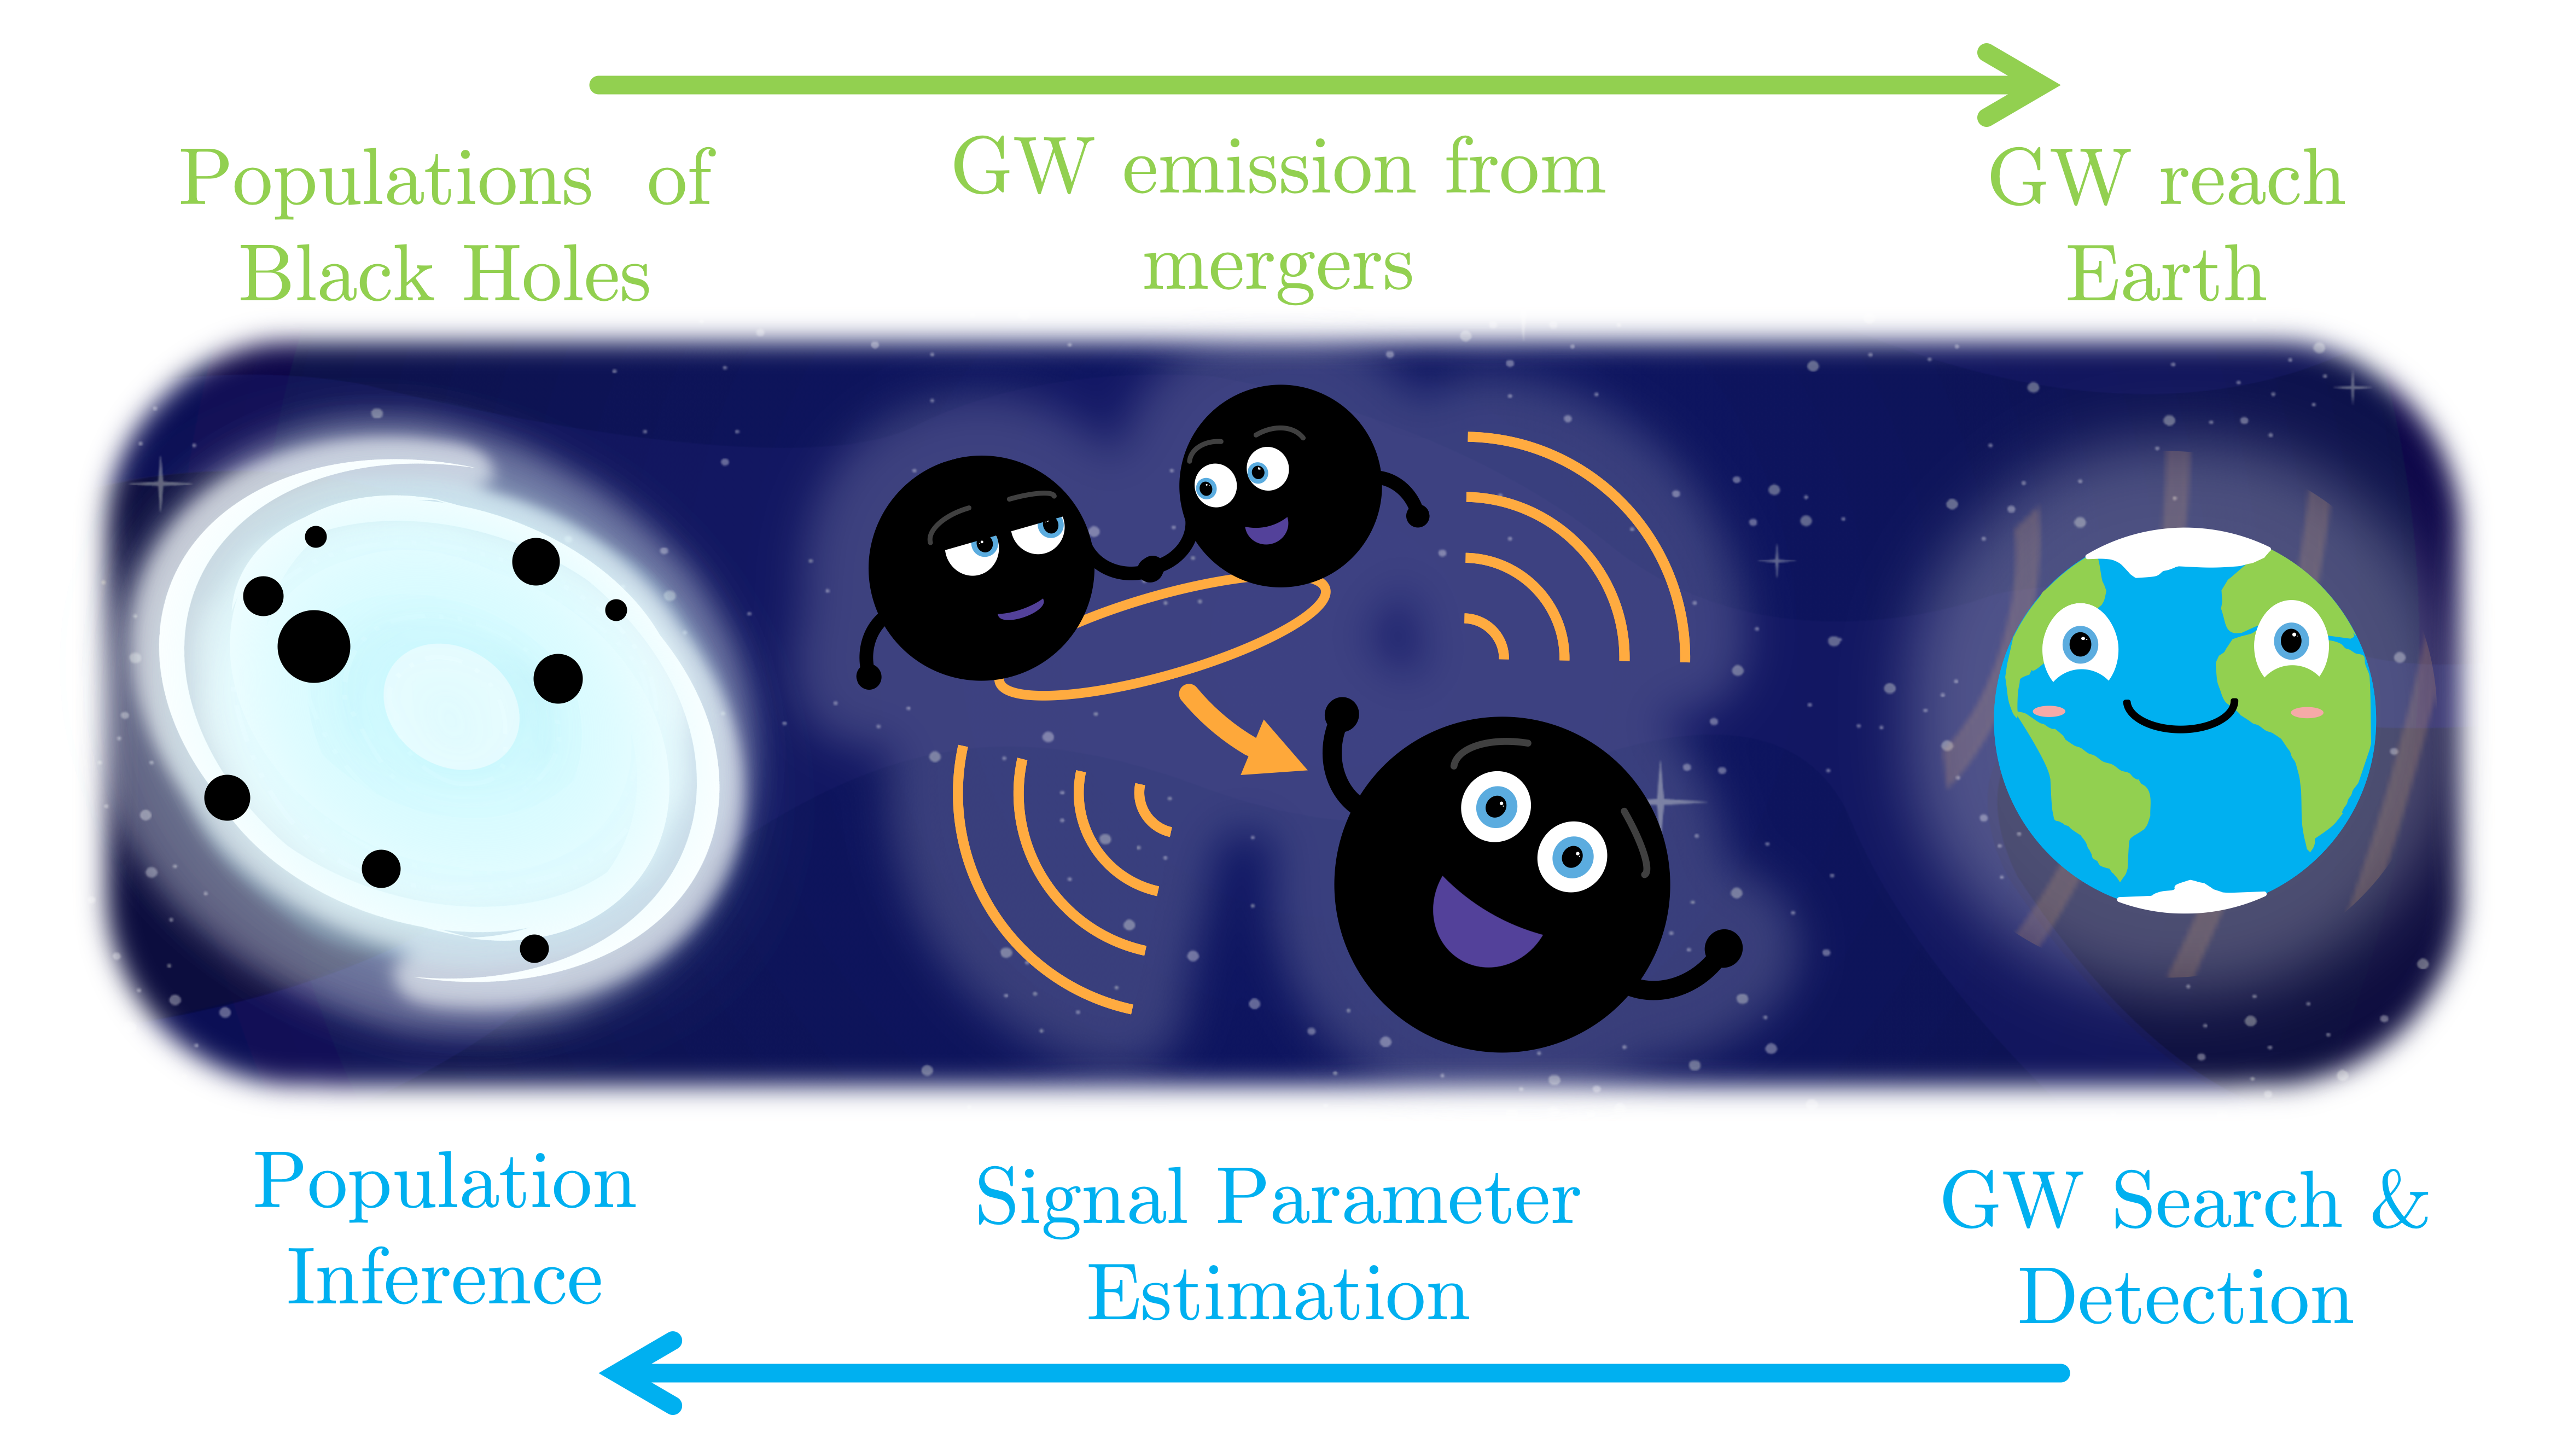
\includegraphics[width=1.1\linewidth]{src/figures/gw_pipeline.png}}
  \caption{\textbf{GW pipeline:} \todo{Remove faces from this schematic} }
  \label{fig:gw_pipeline}
\end{center}
\end{figure}



\subsection{GW searches}  \label{sec:searches}

As LIGO records data, the data is immediately searched for generic, unmodelled GW transients and modeled GW signals using low-latency search pipelines. 
These searches can identify candidate GW events in near real-time timescales, enabling the possibility of performing follow-up electromagnetic spectrum observations~\cite{abbott2018prospects}.

The unmodeled gravitational wave searches, like the Coherent Wave-Burst (cWB) and BayesWave pipelines, are performed without prior information about expected signal waveforms and instead involve cross-correlating the LIGO and Virgo detector data. 
The cross-correlation is performed on the detector strain time series to look for excess power or bursts in the overlap region between the LIGO Hanford and LIGO Livingston detectors and between the LIGO Hanford and Virgo detectors, respectively \cite{LSC:2016}. 
Such methods are effective at identifying GW transients that can last for
$10^{-3}-10^{1}$s~\cite{abbott2016observing}. 
Unmodeled gravitational wave searches are powerful tools as they may help detect short-duration signals produced by unknown and known phenomena for which we have not yet developed good theoretical models~\cite{Abbott:2016blz}. 
For example, short-duration signals from high mass binary black hole mergers, supernovae, cosmic strings, and unknown astrophysical phenomena as described in~\citep{abbott2018prospects}.

While unmodeled searches look for the unknown,  modeled or targeted gravitational wave searches look for signals from known sources~\cite{abbott2016ligo}. 
Modeled searches for GW signals from the coalescence of compact binary coalescence (CBCs), such as `pyCBC'~\cite{biwer2019pycbc} and
`GstLAL' pipelines~\cite{sachdev2019gstlal},  use prior information about our expectations of GWs in searches. These searches compute the inner product between a gravitational waveform and the data stream and attempt to optimize the inner product by testing different waveforms. 
The different waveforms are chosen from a ``template-bank'' of potential waveforms, where each waveform corresponds to different signal parameters. 


These search methods have been able to successully identify more than 90 CBC GWs, whose masses are plotted in Figre~\ref{}.
If the detector data contained only gaussian noise and the occasional gravitational wave signal, these search pipelines would successfully identify all signals above some signal-to-noise ratio. 
Unfortunately, some instrumental noise artifacts (glitches) can also be found in the detector data. 
The search pipelines can mistake `glitches' as gravitational wave signals. 
Hence, the search pipelines also test signal coherence and compute `ranking statistics' to determine the statistical significance of candidates to prevent false positives. 

Efficient signal detection requires a ranking statistic that extracts the most information from the data to discriminate between noise and weak astrophysical signals.  
However, existing CBC searches are not optimal: they do not incorporate knowledge of all features that may distinguish GWs from noise. 
Moving toward an optimal statistic is a great challenge, but one toward a better ranking statistic may be to demand that foreground triggers in two or more detectors should be better described
as coherent gravitational-wave signals rather than incoherent glitches.
Importantly, it is not enough to provide some measure of coherence: one must also prove that an incoherent model is not more successful at
describing the data. 

The Bayesian coherence ratio, `BCR', proposed by \citet{bcr_paper} can help take a step towards this optimal statistic. 
As short-duration gravitational wave signals such as those from intermediate-mass black holes are the most challenging to distinguish from glitches, in Chaper~\ref{cp:imbh}, we investigate the usefulness of the `BCR' as a ranking statistic. 

\subsection{GW Signal Parameter Estimation}

The core of parameter estimation in gravitational waves is Bayes' theorem. 
Given a model with parameters $\theta$, some data $d$ and the \textit{likelihood} $\mathcal{L}(d|\theta)$ of the data given the model, Bayes' theorem states that the \textit{posterior probability} $p(\theta|d)$ of model parameters given the data is 
\begin{equation}
{p(\theta|d)} = \frac{\mathcal{L}(d|\theta)\pi(\theta)}{\mathcal{Z}}\ , \label{eq:bayeTheorem}
\end{equation}
where $\pi(\theta)$ is the \textit{prior} probability of the model parameters, and $\mathcal{Z}$ is the marginalized likelihood known as the
\textit{evidence}. 
The evidence is a single number that describes how well a model fits the data and is given by 
\begin{equation}
Z(d) = \int_\theta \mathcal{L}(d|\theta)\pi(\theta)d\theta\ .
\label{eq:evid}
\end{equation}
As the evidence is a probability of the data irrespective of model parameters, it is a valuable quantity to compare various models and determine which model better describes some data.

Using gravitational wave models and equation~\ref{eq:bayes}, astronomers can compute the posterior probability of gravitational wave model parameters given some data containing a gravitational wave signal~\cite{abbott2018prospects}.
However, as CBC GW models can use more than 11 parameters to describe a signal, evaluating the posterior probability for gravitational waves is computationally expensive. 
For example, consider evaluating the posterior probability at $10$ gridpoints for each of the $11$ GW parameters.
This case results in a huge number of $10^11$ points to evaluate the posterior.
Furthermore, one would need to use many more grid points to represent the continuous parameter space accurately.
Finally, gravitational wave models incorporate complex physics, so they can be computationally slow to evaluate. 
Altogether, evaluating the posterior overall points of parameter space is an insurmountable computational challenge.

An alternative way to estimate the posterior over a large parameter space is to utilize approaches such as Markov chain Monte Carlo (MCMC) and Nested Sampling to produce multivariate draws from the posterior. 
These methods can also be parallelized to speed up the inference process. 
For a detailed discussion on the parallelization of nested sampling and how it can boost gravitational wave inference, refer to Chapter~\ref{cp:pbilby}. 


\begin{figure}
\begin{center}
  \centerline{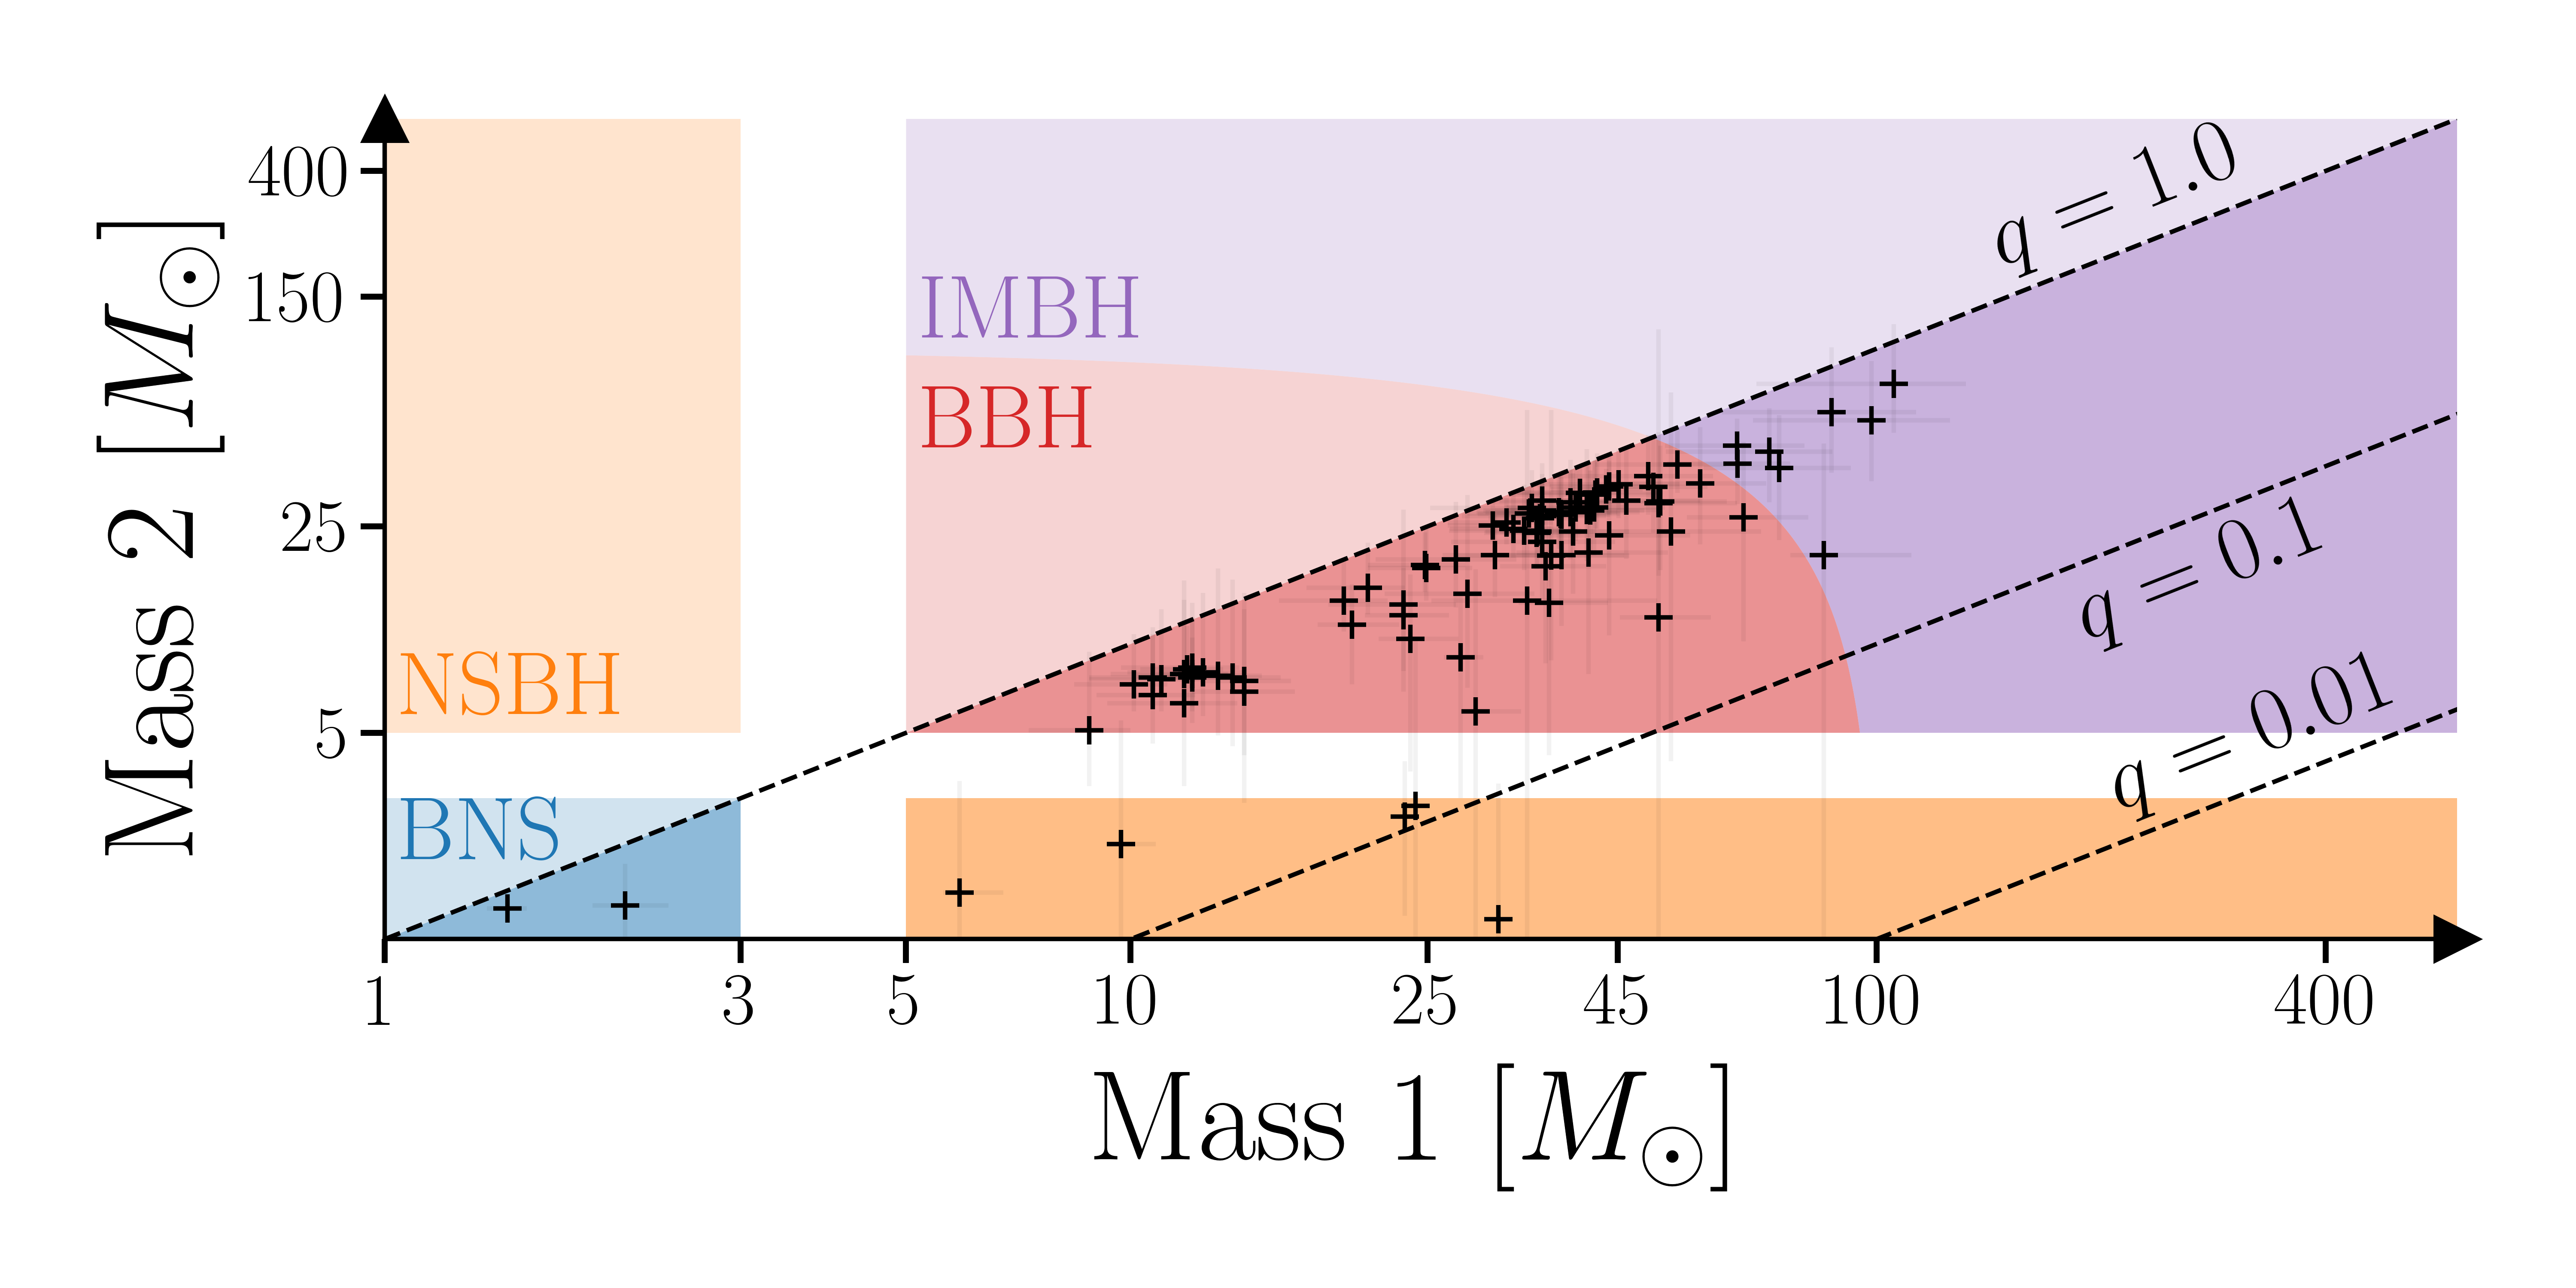
\includegraphics[width=1.1\linewidth]{src/figures/gw_catalog.png}}
  \caption{\textbf{CBC GW merger events:}  \github{https://github.com/avivajpeyi/cbc_gw_catalog_plotter}}
  \label{fig:cbc_mergers}
\end{center}
\end{figure}

\subsection{Interpretting GW signals}

After the CBC GW searches identify signals and parameter estimation pipelines describe the properties of the merging binaries that generated the signals, astronomers can begin interpretting the implications of the various binaries discovered.
The mass and spin deductions of the merging systems can help us answer: where do these bodies exist in the cosmos? 
Do they exist in the centers of active galaxies, or in isolated space?
Each GW observation and the inferred parameters can provide insight into the formation channel that led to the binary's current configuration.

For example, parameter estimation of GW190521 indicate that the signal orginated from an asymmetric binary black hole merger with masses of $85^{+21}_{-14}M_{\odot}$ and $66^{+17}_{-18}M_{\odot}$ and a total mass of $151^{+32}_{-28}M_{\odot}$ \citep{Abbott:2020tfl}.
The remnant object was an IMBH with a total mass exceeding the pulsational-pair instability mass gap.
Another example is the parameter estimation of GW190425. 
\citep{}'s analysis using an eccentric waveform demoonstrates that this event may have occured ini XXX.

In a similar vein, the community has recently been discussions GW151226. Initial work deduced that this GW was from the merger of two black holes (BHs), both with standard masses and spins (case A). However, recent work has deduced that the GW might have originated from a strange system: one BH could be much larger than the other and with a faster spin (case B)! A diagram representing these cases can be seen below on the right side of Figure 1.



But, it gets tricky to answer such questions if our deductions of the masses and spins are incorrect! So, in my recent study, I have built a "deep follow-up" tool to determine which masses and spins better describe a given GW event. 


The "deep follow-up" method involves drilling into these cases to determine which binary BH system better describes the GW. First, we pin down some deduced properties of the merging black hole system, such as the mass-ratio q (the ratio of smaller BH mass divided by the bigger BH mass) and xeff (the effective spin of the binary in the z-direction). The pinned value for the initial and new results is on the left side of Figure 1. We then use Bayesian inference at these pinned values. The output allows us to compare case A and case B. We find that both the standard (case A) and irregular (case B) black hole pairs can describe GW151226, giving the event something like a dual-identity! 

This method is descriebed in paper 2. 


\subsection{GW population inferenc}

Finally, 
The Universe contains different ``flavours'' of black holes. While ``stellar'' mass black holes are 10-50 times the mass of our Sun, supermassive black holes are millions and billions of times the mass of our Sun (like the one in interstellar)! Supermassive black holes (SMBH) are so big that they manage to -- quite literally -- become the centres of their galaxies. Their gravity pulls in celestial bodies like stars, neutron stars and smaller black holes into orbit around them (illustrated in Figure 1). 

The gravitational force also pulls in surrounding gas and dust into a spiralling orbit with an inevitable end in the SMBH. As the gas spirals in, it gets hot due to friction and can even generate bright "jets" of radiation. The spiralling gas is known as an accretion disk, and these can be very thick and even hide some of the celestial bodies inside. Unfortunately, what goes on between bodies inside accretion disks is hidden from us -- our eyes cannot see through these gassy curtains. However, gravitational waves from the mergers of these bodies help spill the beans: they pass through the gassy curtain and let us study both the accretion disk and merging bodies!
 
Scientists have been simulating bodies inside accretion disks to understand how many mergers can happen inside these disks and what the orientations of the bodies are before merging. Based on these simulations, we have constructed a "model" to study the accretion disks' age and density (ie, if the disk is dilute or viscous) from the gravitational waves shot off from the mergers! A visual representation of the model is in Figure 2. 
Figure 2
 
Active galactic nuclei (AGN) are promising environments for the assembly of merging binary black hole (BBH) systems. Interest in AGNs as nurseries for merging BBH is rising following the detection of gravitational waves from a BBH system from the purported pair-instability mass gap, most notably, GW190521. Active galactic nuclei have also been invoked to explain the formation of the high-mass-ratio system, GW190814. We draw on simulations of BBH systems in AGN to propose a phenomenological model for the distribution of black hole spins of merging binaries in AGN disks. The model incorporates distinct features that make the AGN channel potentially distinguishable from other channels such as assembly in the field and in globular clusters. The model parameters can be mapped heuristically to the age and density of AGN disks. We estimate the extent to which different populations of mergers in AGNs can be distinguished. If the majority of merging black holes are assembled in AGNs, future gravitational-wave observations may provide insights into the dynamics of AGN disks.






\section{The hunt for exoplanets

Humans have long sought for exoplanets, or planets beyond our solar system. In recent years, advances in technology have allowed us to find and study many exoplanets. We have now found thousands of exoplanets, and we are learning more about them every day.

There are many different types of exoplanets, and they can be very different from the planets in our solar system. Some exoplanets are very large, while others are very small. Some exoplanets are very close to their star, while others are very far away. And some exoplanets are very hot, while others are very cold.

Despite these differences, there are some things that all exoplanets have in common. All exoplanets orbit a star, and all exoplanets are made of the same basic materials as the planets in our solar system.

This section reviews the 

\begin{itemize}
    \item History: We have looked for exoplanets for along time, first few exoplanets found 
    \item Plot of detectiions vs time
    \item categories of exoplanets + Habitable zone
    \item radius + mass info relations of exoplanets 
    \item Kepler project -- cone in sky
    \item now, TESS project, helped us find many more, survey satellite for nearby stuff
    \item gist of search pipeline + parameters provided
    \item our work 
\end{itemize}



\begin{figure}
\begin{center}
  \centerline{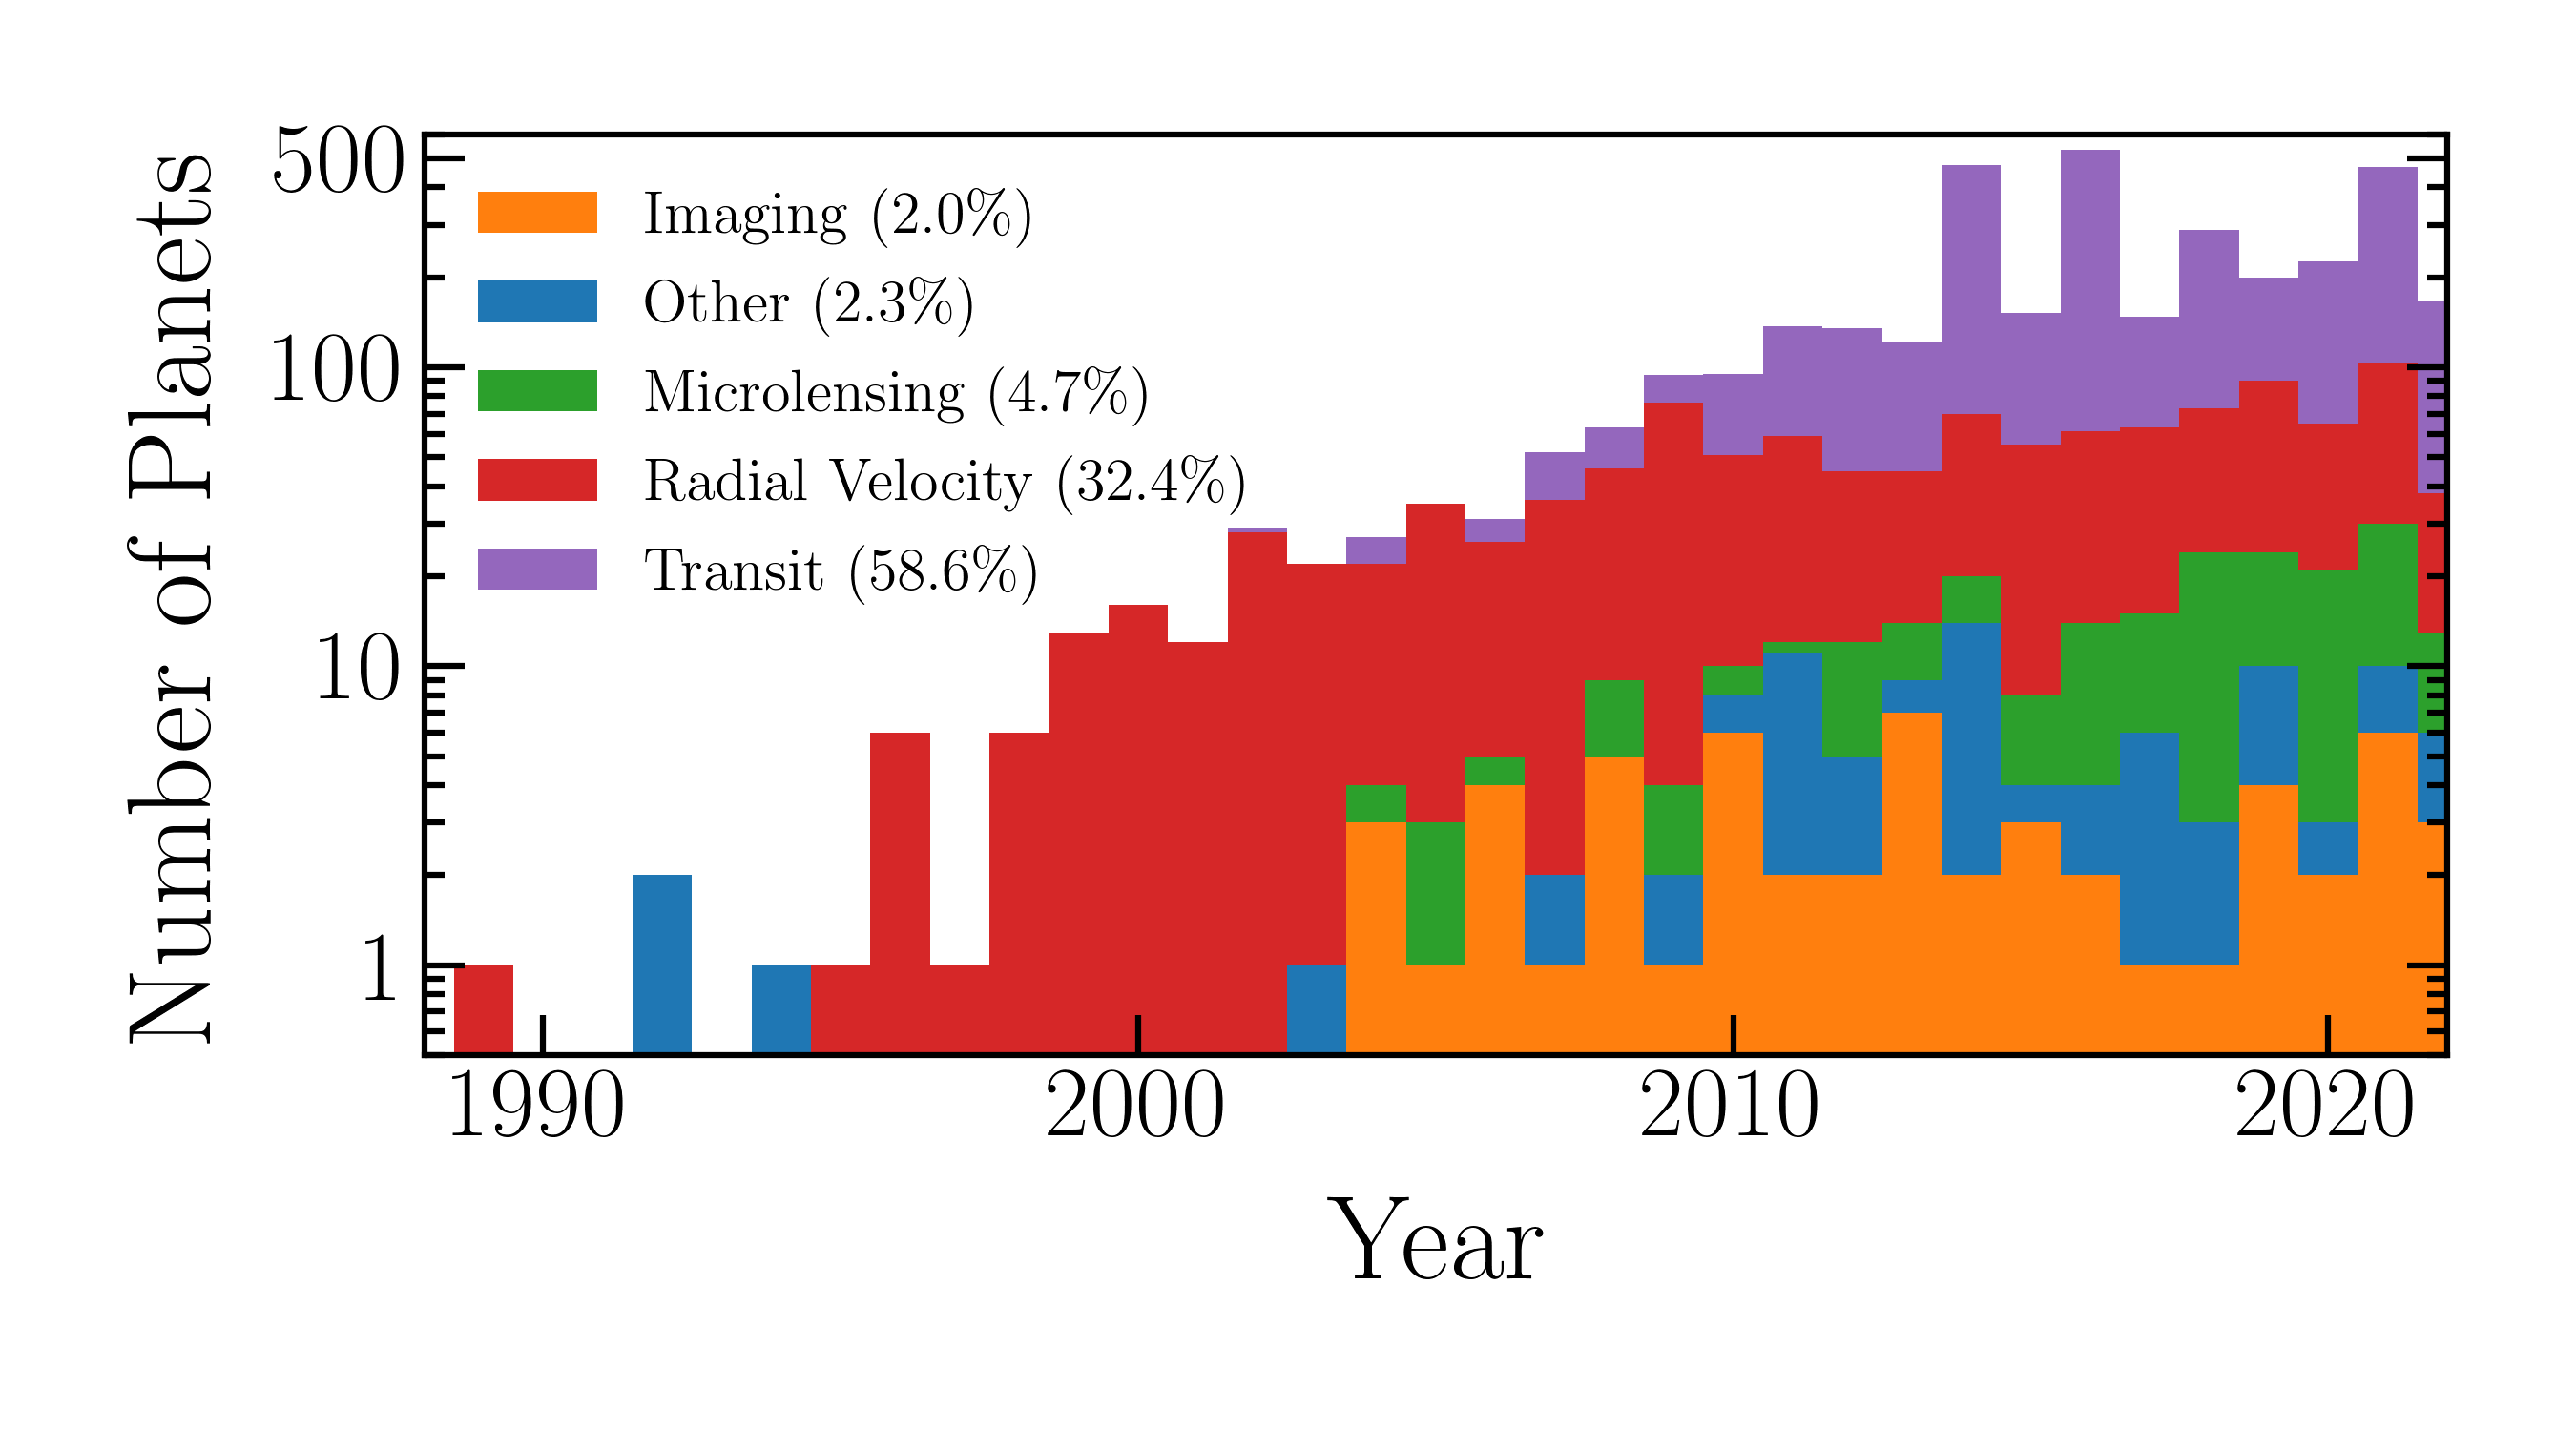
\includegraphics[width=1.\linewidth]{src/figures/confirmed_planets_vs_time.png}}
  \caption{\textbf{Exoplanet detections over time:}  \github{https://github.com/avivajpeyi/exoplanet_catalog_plotter}}
  \label{fig:exo_detections_over_time}
\end{center}
\end{figure}


\begin{figure}
\begin{center}
  \centerline{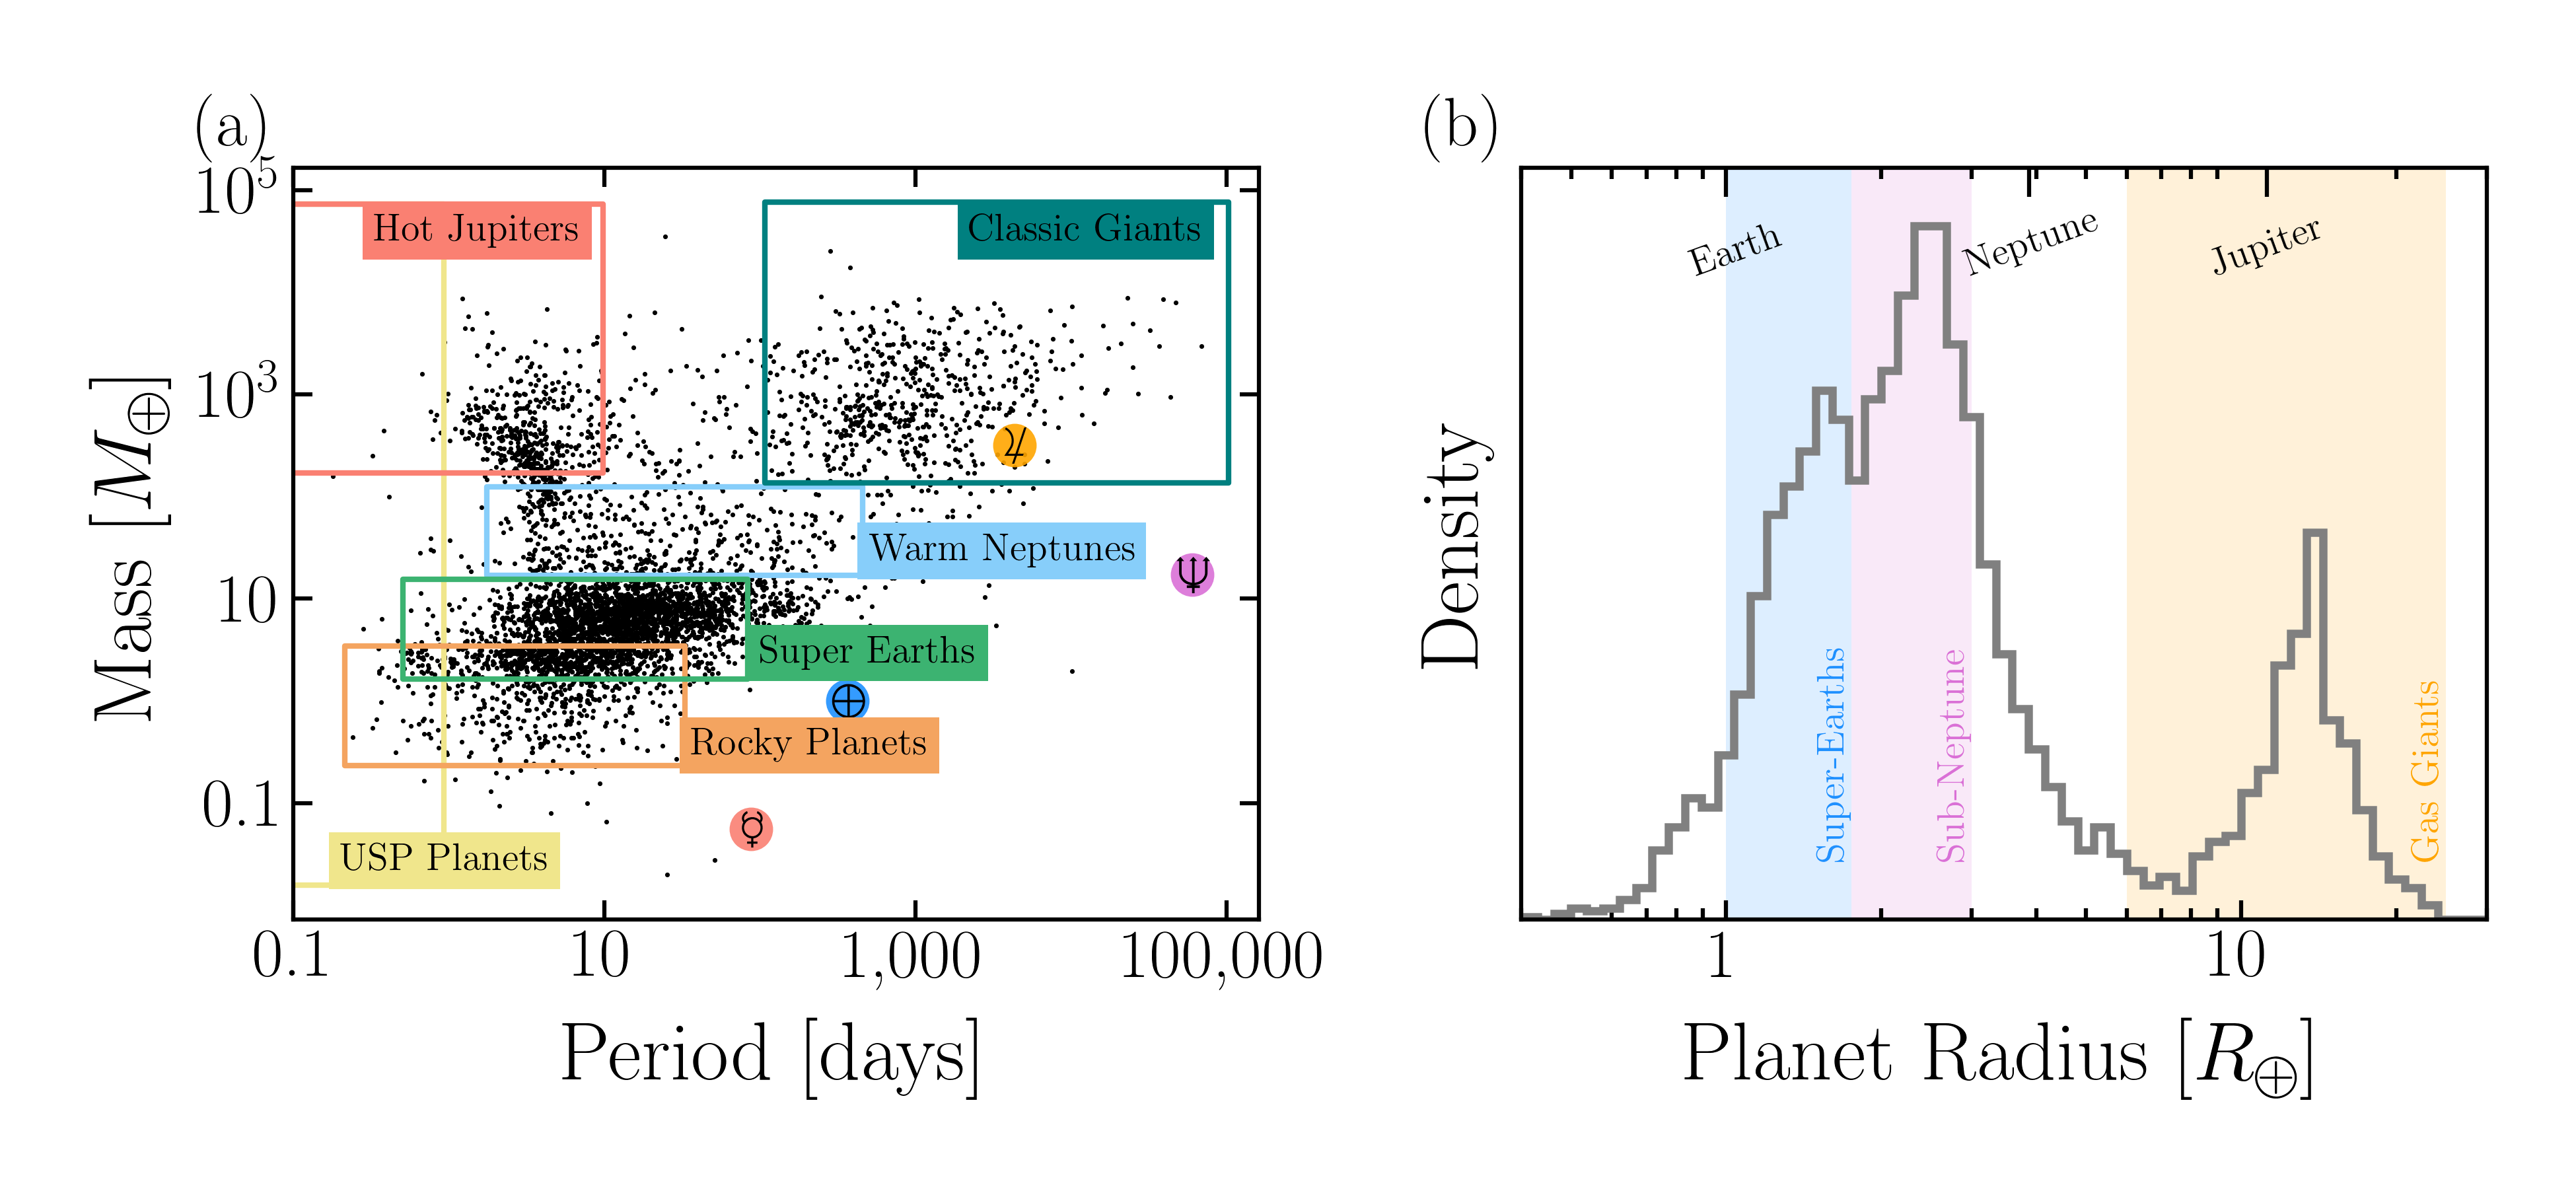
\includegraphics[width=1.\linewidth]{src/figures/scatter_categories.png}}
  \caption{\textbf{Exoplanet Categories:}  \github{https://github.com/avivajpeyi/exoplanet_catalog_plotter}}
  \label{fig:exo_categories}
\end{center}
\end{figure}


\begin{figure}
\begin{center}
  \centerline{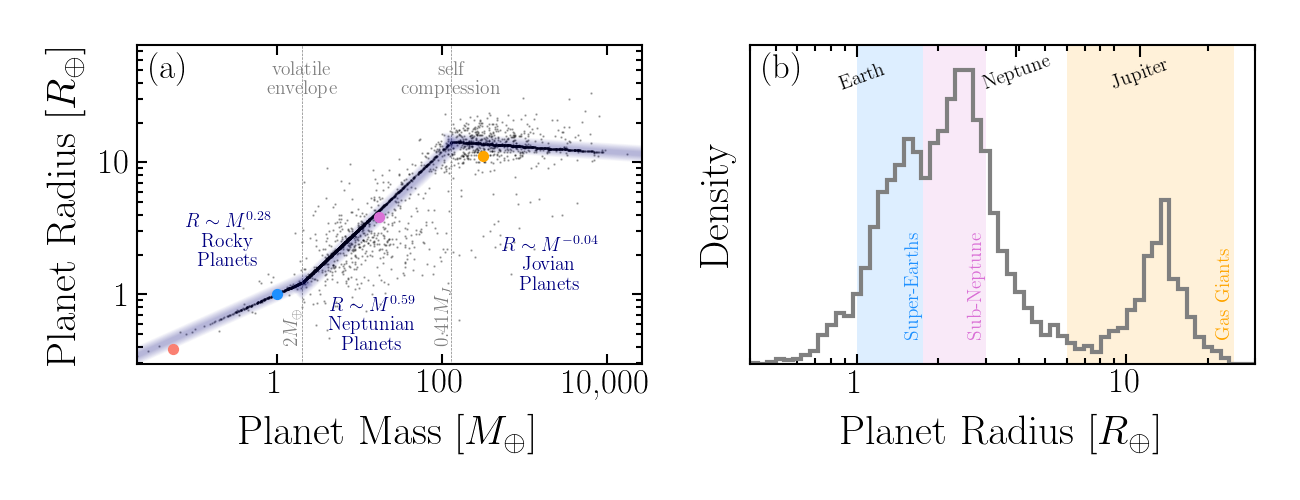
\includegraphics[width=1.\linewidth]{src/figures/radii_and_mass_relations.png}}
  \caption{\textbf{Digging into exoplanet mass and radius distributions:}  \github{https://github.com/avivajpeyi/exoplanet_catalog_plotter}}
  \label{fig:exo_mass_radius_relations}
\end{center}
\end{figure}




% Rocky vs gas 
% http://backalleyastronomy.blogspot.com/2013/07/au-dela-de-neuf-cents-exoplanetes.html
